\chapter{楽曲制作}
\section{NoteSequenceの作成}
NoteSequenceとはMIDIデータから作成されるプロトコルバッファである.
プロトコルバッファとはGoogleは2008年にオープンソース化したスキーマ言語であり,スキーマ言語とは.
MagentaはPythonで作成されているので,実行するにはPythonファイルを指定し実行するか,
NoteSequenceの作成は図のコマンドで作成できる.
\begin{figure}[!ht]
    \begin{screen}
    \begin{center}
        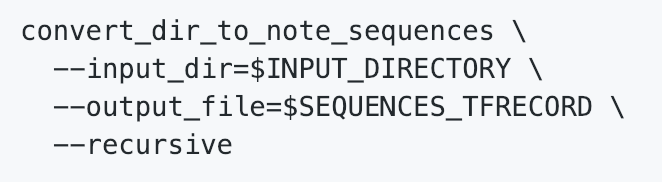
\includegraphics[scale=0.7, clip]{./img/Notesequence_make.png}
        \caption{NoteSequenceの作成}
        \label{fig:NoteSequenceの作成}
    \end{center}
    \end{screen}
\end{figure} \\
--inputdirで学習させるMIDIデータの 絶対パスを指定し,--outputfileでNotesequenceの出力先のディレクトリを指定する.\\
次に作成したNoteSequenceのデータセットを学習用と評価用に分割するために,下記のコマンドを実行する.
\begin{figure}[!ht]
    \begin{screen}
    \begin{center}
        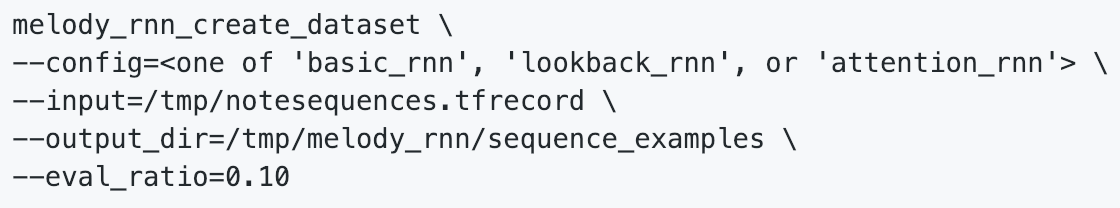
\includegraphics[scale=0.7, clip]{./img/Notesequence_split.png}
        \caption{NoteSequenceを学習用と評価表に分割}
        \label{fig:NoteSequenceを学習用と評価表に分割}
    \end{center}
    \end{screen}
\end{figure}\\
--configで使用するRNNを指定する.--evalratioでNotesequenceの10%が評価のためのデータになり,残りの90%が学習用のデータになる.\\
\newpage
\subsection{学習の開始}
\begin{figure}[!ht]
    \begin{screen}
    \begin{center}
        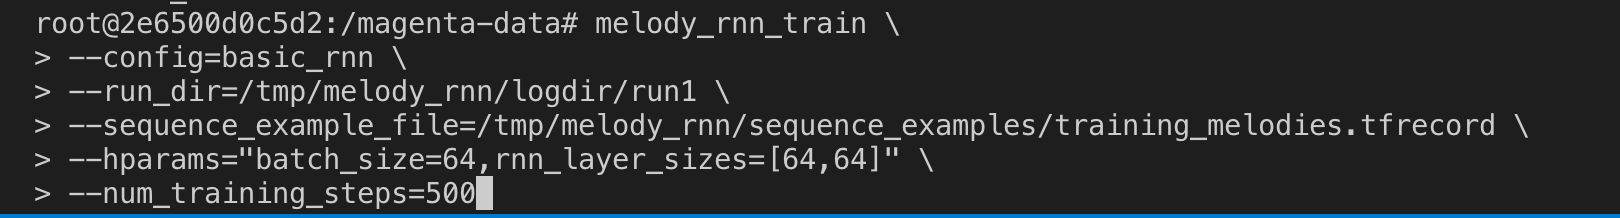
\includegraphics[scale=0.5, clip]{./img/Rnn_train.png}
        \caption{BasicRNNを使用した学習の開始}
        \label{fig:BasicRNNを使用した学習の開始}
    \end{center}
    \end{screen}
\end{figure}
--configで学習に使用する学習モデルを指定,--rundirで,--sequenceexamplefileで学習のために用意したNotesequenceを指定する.
--hparamsでメモリの使用量を指定し,--rnnlayersizeで中間層のノード数を指定し,--numtrainingstepsで学習回数を設定する.\\
\begin{figure}[!ht]
    \begin{screen}
    \begin{center}
        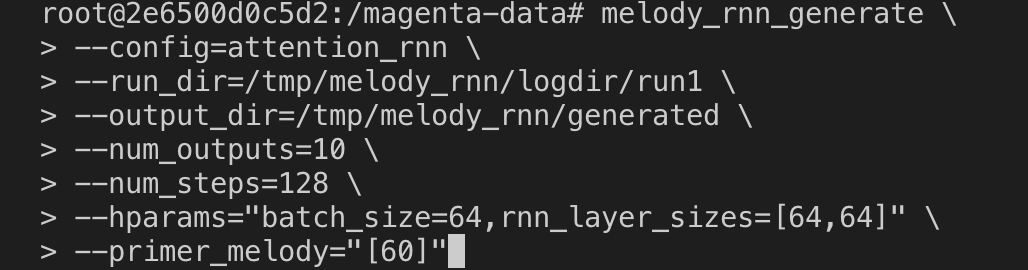
\includegraphics[scale=0.5, clip]{./img/MIDI_make.png}
        \caption{学習モデルを使用し,10曲を作成}
        \label{fig:学習モデルを使用し,10曲を作成}
    \end{center}
    \end{screen}
\end{figure}

\section{PolyfonyRNN}